%---------------------------------------------------------------------------%
%-                                                                         -%
%-                           LaTeX Template                                -%
%-                                                                         -%
%---------------------------------------------------------------------------%
%- Copyright (C) Huangrui Mo <huangrui.mo@gmail.com> 
%- This is free software: you can redistribute it and/or modify it
%- under the terms of the GNU General Public License as published by
%- the Free Software Foundation, either version 3 of the License, or
%- (at your option) any later version.
%---------------------------------------------------------------------------%
%->> Document class declaration
%---------------------------------------------------------------------------%
\documentclass[twoside]{Style/ucasthesis}%
%- Multiple optional arguments:
%- [<oneside|twoside|print>]% oneside eprint, twoside eprint, or paper print
%- [fontset=<adobe|none|...>]% specify font set instead of automatic detection
%- [scheme=plain]% thesis writing of international students
%- [draftversion]% show draft version information
%- [standard options for ctex book class: draft|paper size|font size|...]%
%---------------------------------------------------------------------------%
%->> Document settings
%---------------------------------------------------------------------------%
\usepackage[authoryear,list]{Style/artratex}% document settings
%- usage: \usepackage[option1,option2,...,optionN]{artratex}
%- Multiple optional arguments:
%- [bibtex|biber]% set bibliography processor and package
%- [<numbers|super|authoryear|alpha>]% set citation and reference style
%- <numbers>: textual: Jones [1]; parenthetical: [1]
%- <super>: textual: Jones superscript [1]; parenthetical: superscript [1]
%- <authoryear>: textual: Jones (1995); parenthetical: (Jones, 1995)
%- <alpha>: textual: not available; parenthetical: [Jon95]
%- [geometry]% reconfigure page layout via geometry package
%- [lscape]% provide landscape layout environment
%- [xhf]% disable header and footer via fancyhdr package
%- [color]% provide color support via xcolor package
%- [background]% enable page background
%- [tikz]% provide complex diagrams via tikz package
%- [table]% provide complex tables via ctable package
%- [list]% provide enhanced list environments for algorithm and coding
%- [math]% enable some extra math packages
%- [xlink]% disable link colors
\usepackage{Style/artracom}% user defined commands
%---------------------------------------------------------------------------%
%->> Document inclusion
%---------------------------------------------------------------------------%
%\includeonly{Tex/Chap_1,...,Tex/Chap_N}% selected files compilation
%---------------------------------------------------------------------------%
%->> Document content
%---------------------------------------------------------------------------%
%-
%-> Titlepage information
%-
%---------------------------------------------------------------------------%
%->> Titlepage information
%---------------------------------------------------------------------------%
%-
%-> 中文封面信息
%-
\confidential{}% 密级:只有涉密论文才填写
\schoollogo[scale=0.095]{ucas_logo}% 校徽
\title{DeepDark: 一款高性能缓存生成器设计}% 论文中文题目
\author{刘志刚}% 论文作者
\advisor{孙凝晖~研究员}% 指导教师:姓名 专业技术职务 工作单位
%\advisor{指导教师一\\指导教师二\\指导教师三}% 多行指导教师示例
\degree{硕士}% 学位:学士、硕士、博士
\degreetype{工学}% 学位类别:理学、工学、工程、医学等
\major{计算机系统结构}% 二级学科专业名称
\institute{中国科学院计算技术研究所}% 院系名称
%\institute{中国科学院力学研究所\\流固耦合实验室}% 多行院系名称示例
\date{2020~年~6~月}% 毕业日期:夏季为6月、冬季为12月
%-
%-> 英文封面信息
%-
\TITLE{DeepDark: A High Performance Cache Generator}% 论文英文题目
\AUTHOR{Zhigang Liu}% 论文作者
\ADVISOR{Supervisor: Professor Ninghui Sun}% 指导教师
\DEGREE{Master}% 学位:Bachelor, Master, Doctor, Postdoctor。封面据英文学位名称自动切换,需确保拼写准确
\DEGREETYPE{Engineering}% 学位类别:Philosophy, Natural Science, Engineering, Economics, Agriculture 等
\MAJOR{Computer Systems Organization}% 二级学科专业名称
\INSTITUTE{Institute of Computing Technology, Chinese Academy of Sciences}% 院系名称
\DATE{June, 2020}% 毕业日期:夏季为June、冬季为December
%---------------------------------------------------------------------------%
%
\begin{document}
%-
%-> Frontmatter: title page, abstract, content list, symbol list, preface
%-
\frontmatter% initialize the environment
%---------------------------------------------------------------------------%
%->> Frontmatter
%---------------------------------------------------------------------------%
%-
%-> 生成封面
%-
\maketitle% 生成中文封面
\MAKETITLE% 生成英文封面
%-
%-> 作者声明
%-
\makedeclaration% 生成声明页
%-
%-> 中文摘要
%-
\intobmk\chapter*{摘\quad 要}% 显示在书签但不显示在目录
\setcounter{page}{1}% 开始页码
\pagenumbering{Roman}% 页码符号

本文是中国科学院大学学位论文模板ucasthesis的使用说明文档。主要内容为介绍\LaTeX{}文档类ucasthesis的用法,以及如何使用\LaTeX{}快速高效地撰写学位论文。

\keywords{中国科学院大学,学位论文,\LaTeX{}模板}% 中文关键词
%-
%-> 英文摘要
%-
\intobmk\chapter*{Abstract}% 显示在书签但不显示在目录

This paper is a help documentation for the \LaTeX{} class ucasthesis, which is  a thesis template for the University of Chinese Academy of Sciences. The main content is about how to use the ucasthesis, as well as how to write thesis efficiently by using \LaTeX{}.

\KEYWORDS{University of Chinese Academy of Sciences (UCAS), Thesis, \LaTeX{} Template}% 英文关键词
%---------------------------------------------------------------------------%
% title page, abstract
{% content list region
\linespread{1.2}% local line space
\intobmk*{\cleardoublepage}{\contentsname}% add link to bookmark
\tableofcontents% content catalog
\intobmk*{\cleardoublepage}{\listfigurename}% add link to bookmark
\listoffigures% figure catalog
\intobmk*{\cleardoublepage}{\listtablename}% add link to bookmark
\listoftables% table catalog
}
\intobmk\chapter*{符号列表}% 显示在书签但不显示在目录

\section*{字符}
\nomenclatureitem[\textbf{Unit}]{\textbf{Symbol}}{\textbf{Description}}
\nomenclatureitem[$\Unit{m^{2} \cdot s^{-2} \cdot K^{-1}}$]{$R$}{the gas constant}
\nomenclatureitem[$\Unit{m^{2} \cdot s^{-2} \cdot K^{-1}}$]{$C_v$}{specific heat capacity at constant volume}
\nomenclatureitem[$\Unit{m^{2} \cdot s^{-2} \cdot K^{-1}}$]{$C_p$}{specific heat capacity at constant pressure}
\nomenclatureitem[$\Unit{m^{2} \cdot s^{-2}}$]{$E$}{specific total energy}
\nomenclatureitem[$\Unit{m^{2} \cdot s^{-2}}$]{$e$}{specific internal energy}
\nomenclatureitem[$\Unit{m^{2} \cdot s^{-2}}$]{$h_T$}{specific total enthalpy}
\nomenclatureitem[$\Unit{m^{2} \cdot s^{-2}}$]{$h$}{specific enthalpy}
\nomenclatureitem[$\Unit{kg \cdot m \cdot s^{-3} \cdot K^{-1}}$]{$k$}{thermal conductivity}
\nomenclatureitem[$\Unit{kg \cdot m^{-1} \cdot s^{-2}}$]{$S_{ij}$}{deviatoric stress tensor}
\nomenclatureitem[$\Unit{kg \cdot m^{-1} \cdot s^{-2}}$]{$\tau_{ij}$}{viscous stress tensor}
\nomenclatureitem[$\Unit{1}$]{$\delta_{ij}$}{Kronecker tensor}
\nomenclatureitem[$\Unit{1}$]{$I_{ij}$}{identity tensor}

\section*{算子}
\nomenclatureitem{\textbf{Symbol}}{\textbf{Description}}
\nomenclatureitem{$\Delta$}{difference}
\nomenclatureitem{$\nabla$}{gradient operator}
\nomenclatureitem{$\delta^{\pm}$}{upwind-biased interpolation scheme}

\section*{缩写}
\nomenclatureitem{CFD}{Computational Fluid Dynamics}
\nomenclatureitem{CFL}{Courant-Friedrichs-Lewy}
\nomenclatureitem{EOS}{Equation of State}
\nomenclatureitem{JWL}{Jones-Wilkins-Lee}
\nomenclatureitem{WENO}{Weighted Essentially Non-oscillatory}
\nomenclatureitem{ZND}{Zel'dovich-von Neumann-Doering}

% symbol list, preface content
%-
%-> Mainmatter
%-
\mainmatter% initialize the environment
%---------------------------------------------------------------------------%
%->> Main content
%---------------------------------------------------------------------------%
\chapter{引言}\label{chap:introduction}


\section{研究背景}

随着诸如Dennard Scaling和摩尔定律等传统工艺技术演进所带来的收益的大大减少,计算机体系结构有望进入创新的黄金时代。领域专用架构(DSA)是一种有前途的解决方案,可以继续提高计算性能,同时能向以前工艺演进一样,带来能量和面积效率水平的极大提升。不幸的是,传统的芯片设计方法和硬件开发方法需要大量的非经常性工程成本(NRE成本),包括工具,人工,IP和时间等。这极大提升了芯片设计的门槛,最终阻碍了DSA的广泛采用。

而与之相对应的是,由于开源软件的激增,过去几十年软件开发的大量工程成本和极长的设计周期已大大缩减。一个小型的软件开发团队现在可以针对他们自己的用户群体的需求,使用更高级的工具,迅速实现他们创新的想法。受到软件社区的启发,开放式的硬件设计被认为是降低芯片设计成本的最有前途的方法之一,受到了学术界和工业界的普遍关注。对于学术界来说,与开源软件模拟器(例如gem5,MARSSx86,Sniper或ZSim)相比,开源硬件实现具有许多优势。与软件模型不同,硬件实现可以演示精确的微体系结构行为,运行包含大量指令数的实际应用程序,并凭提供功率和面积测量结果。此外,开放式硬件实现还提供了一个基准平台,作为新微体系结构优化的baseline。对工业界来说,开放的硬件标准意味着他们可以共建共享复杂的软件或硬件生态,而不必被标准专利构筑的门槛拦在市场之外。开放的硬件实现,则可以降低了他们的IP开发成本,缩短设计周期。

最近一些年,涌现出了大量开源芯片设计的工作,开源芯片设计的生态逐渐繁荣。处理器核,cache,外设,加速器,SoC等,都有了开源的设计实现。我们以Chipyard SoC集成框架为例,展示开源芯片生态的现状。Chipyard是用于对硬件进行全系统的设计和评估的一套框架。它包含了一系列工具、库以及开源IP,可以将现有的开源芯片设计以及商业的芯片设计整合成一个完整的SoC。
Chipyard包含有以下IP和模块:

\begin{center}
    \begin{tabular}{lp{12cm}}
        \hline
			类别 & 项目/IP\\
        \hline
			处理器核 & RocketCore(顺序单发射处理器核),BOOM core(乱序多发射处理器核)\\
        \hline
			缓存 & Sifive BlockInclusiveCache,TLSimpleL2\\
        \hline
			多核 & Rocketchip(SoC框架)\\
        \hline
			加速器 & Hwacha(向量加速器),Gemmini:(脉动阵列生成器),NVLDA(AI推理加速器),SHA3 RoCC Accelerator(SHA3哈希算法加速器)\\
        \hline
			设备 & IceNet(NIC),UART,SPI Flash\\
        \hline
			片上网络 & Tilelink SEREES,Switch,Ring Network(NoC)\\
        \hline
    \end{tabular}
\end{center}

可以看出,开源的芯片设计种类基本齐全,使用开源的IP能够组成基本可用的SoC。但是开源IP仍然存在不少的问题,这使得他们更多是用于学术界的实验性流片,而没有在工业界得到广泛使用。开源IP相对于商业IP的劣势主要是在于如下的几个方面:

\begin{enumerate}
	\item 性能差,主要是指PPA(Power Performance,Area)上的差距。例如经我们评估Boom乱序处理器核只能0.9GHz,而商用的ARM乱序处理器核能达到2.8GHz的频率。
	\item 功能不齐全:开源的芯片设计只满足了基本的功能,而对于商用需要的更多功能,则没有实现。例如ECC等特性。
	\item 质量不可靠:开源芯片设计大都没有经过完善的验证,没有配套的验证环境,不满足流片必须的覆盖率质量指标。
\end{enumerate}

开源芯片设计距离高度可用,广泛使用,仍然有很多工作要做。本工作聚焦于缓存部分,希望能产出一款开源的,高度可用的(性能,功能,质量都达标的)的cache生成器,为开源生态的繁荣贡献一份力量。

\section{研究动机}

\subsection{现有cache设计的不足}


尽管最近确实有一些开源的cache设计,例如Sifive BlockInclusiveCache,XXX,TLSimpleL2,XXX。但是它们的性能,质量,通用性都不太好。这阻碍了开源芯片的广泛应用。
这里或许可以上一个表,列出现有的开源的cache在哪些方面有问题。

\subsection{cache设计的挑战}

在本工作中,我们试图解决这个问题,设计实现一个高性能,高质量,开源的cache生成器。设计一款cache生成器存在诸多挑战:

1. 高性能:
  * 延迟,吞吐(现代处理器大多是乱序,多核,这需要大量的MLP,各种预取,替换算法)
  * 延迟,频率
  * 命中率:各种预取,替换算法
2. 高质量:
  cache设计存在大量的复杂性,怎样把它搞对。复杂性体现在:
  * 一致性协议
  * 繁多的请求类型:cache请求,uncache请求,原子操作
  * 复杂的请求处理流程:(这个可以画一个L2的各种case,各种路径做个案例。最好画成树状的,就是我们有多少条不同的请求处理路径)
3. 通用性/灵活性
  现代处理中往往有多个层次的cache,L1,L2,L3,L4等。L1往往与核心是紧耦合的,而其他cache层次,大多与核心松耦合,它们往往有相同的接口:上下都是标准的总线协议,同时有相似的请求处理流程。因此作为一款cache生成器,我们希望它能尽可能地通用,同一份代码,不同的配置,就可以生成满足不同层次需求的cache。通用性带来的挑战主要是L2,L3,L4有不同的延、吞吐的性能需求,怎样用同一份代码满足不同的需求。

\section{论文的主要内容和贡献}

本工作设计实现了一款cache生成器:DeepDark,它是一款高性能,高质量,高灵活性的cache生成器,面向高性能处理器的缓存层次。GAIO以多种方法解决了Cache设计存在的多个挑战。

1. 高性能:
  * 常用路径与非常用路径分开,降低常用路径的延迟。
  * 多MSHR以提升吞吐
  * 与后端紧密结合的设计,确保频率达标
2. 高质量:
  * 基于UVM验证方法学的随机验证框架
  * 系统级测试
3. 高灵活性:
  * 高可配置性
  * 算法插件化,算法可配置

  我们使用chisel编程语言实现了DeepDark,它的延迟为XXX,吞吐达到XXX,在SMIC 14nm工艺下,频率高达2.0GHz。能够支持Linux,XXX等应用。

  易难的意见,贡献这里总结得不够好,可以先写其他的,最后再总结。

总结:本工作做出了三点微小的贡献:
1. 高性能cache的设计与实现
2. cache的验证
3. 高度灵活性,高度可配置,具备高通用性的cache结构设计

\section{论文组织}

本文的后续章节组织结构如下:

第二章介绍了本工作所涉及到的一些工程技术方面的背景知识,包括Tilelink总线协议,芯片验证的基础知识以及业界常用的UVM验证方法学等。这部分背景知识补齐了一些技术细节,帮助读者更好地理解本工作设计、实现以及验证部分的内容。

第三章介绍了DeepDark cache生成器的设计,包括架构设计,在此架构设计下请求的处理流程以及一些性能优化。

第四章介绍了DeepDark的实现。首先介绍了本工作基于的code base以及选用的语言。 接下来介绍了实现上的一些重要细节,例如主要模块的结构,它们的流水级、状态机;重要的同步、一致性协议、transaction control等问题在实现上是如何解决的等。最后还介绍了一些重要算法的实现。

第五章介绍了DeepDark cache生成器的验证。包括了cache需要验证的功能,cache验证的难点,cache验证方案的设计和cache验证环境的实现。

第六章介绍了DeepDark的评估。首先介绍了评估实验的配置以及实验的方法论。然后对cache的性能,后端实现,验证等各方面进行了综合的评估,并给出了结果。

第六章对相关工作进行总结,并展望了下一步的研究方向。

\chapter{背景}\label{chap:background}

第二章介绍了本工作所涉及到的一些工程技术方面的背景知识,包括Tilelink总线协议,芯片验证的基础知识以及业界常用的UVM验证方法学等。这部分背景知识补齐了一些技术细节,帮助读者更好地理解本工作的后续内容。

\section{TileLink一致性协议}

\subsection{TileLink简介}

TileLink是芯片级的互连标准,为多个主设备提供对内存和其他从设备的一致性的内存映射访问。TileLink作为快速可扩展互连协议,可提供低延迟和高吞吐量的传输。它被设计用于在片上系统(SoC)中连接通用多处理器,协处理器,加速器,DMA引擎以及简单或复杂的设备。
TileLink是类似ARM AXI和ACE的,通用的、支持一致性的总线协议以及互联标准。
TileLink的一些重要特性包括:
\begin{enumerate}
	\item 标准免费开放
	\item 为RISC-V设计,但也支持其他的ISA
	\item 为任意的缓存(如处理器核)或非缓存主设备(如DMA master)提供一致性的内存访问,支持类似MESI的一致性协议
\end{enumerate}

这些重要特性,让TileLink在开源芯片设计中广受欢迎。TileLink相关IP(如CrossBar,Arbiter,SerDes,NoC等)齐全并且很成熟,同时大量的开源芯片设计都使用TileLink总线作为访存接口,如Rocket Chip,Boom等。

为了支持各种不同设备从简单到复杂的访存需求,TileLink规范定义了三种协议兼容级别,这些级别说明了设备必须支持协议的哪个子集,如下表所示。
最简单的是TileLink轻量级不缓存(TL-UL),仅支持简单的内存读写(Get/Put)单个字的操作。它可以用于简单的,只需要单个字读写访问的,如UART之类外设。
接下来最复杂的是TileLink重量级不缓存(TL-UH),它添加了各种Hint(提示),原子操作和突发访问,但不支持一致性缓存。它可以用于稍微复杂一点的,需要较高数据吞吐量,同时又不需要自己硬件上维护一致性的主设备,如ICache,DMA master等。
最后,TileLink缓存(TL-C)是完整的协议,它支持使用一致性的缓存。它可以用于完整的,自己维护硬件一致性的cache,如DCache,L2,L3等各级Cache。

TL-UL和TL-UH中的消息,都是master请求slave执行一些读写预取操作,master没有获取数据块的权限,不要求将数据块的所有权从slave转移到master这边。因此它们常常用于master自己不需要缓存数据块(如DMA engine),或者master自己缓存的数据块是软件维护一致性,不需要硬件维护一致性(例如ICache)的情况。由于master并不请求数据块权限以缓存在本地,所以这些请求被称为uncached请求,这也是两个协议名称中U的由来。

TL-UL,TL-UH和TL-C三种兼容性级别,低级别是高级别的真子集,高级别包含了低级别的所有通道,所有消息(低级别的消息在高级别中功能可能会被扩展)。
兼容性级别越高,支持的消息越来越多,支持的功能越来越强。相应的,master和slave端的实现也就更加复杂。


\begin{center}
\begin{tabular}{|l|l|l|l|}
\hline
                      & \textbf{TL-UL} & \textbf{TL-UH} & \textbf{TL-C} \\ \hline
Read/Write operations & $\checkmark$   & $\checkmark$   & $\checkmark$  \\ \hline
Multibeat messages    & $\checkmark$   & $\checkmark$   & $\checkmark$  \\ \hline
Atomic operations     & $\checkmark$   & $\checkmark$   & $\checkmark$  \\ \hline
Hint operations       & $\times$       & $\checkmark$   & $\checkmark$  \\ \hline
Cache block transfers & $\times$       & $\times$       & $\checkmark$  \\ \hline
Channels B+C+E        & $\times$       & $\times$       & $\checkmark$  \\ \hline
\end{tabular}
\end{table}

我感觉应该把channel,message,transaction合并成一页,然后再把coherence搞一页。
关于tilelink,大家主要要理解啥呢?tilelink有哪些流程,它们走的什么通道。每个通道是用来干啥的,就OK了吧?
其他太过于细节的,其实是不必要的啊。

channel上是message,message构成transaction,transaction支持请求的流程。然后对于这些流程,我们只需要着重介绍read/write,还有cache block transfer就好了吧。
这个应该怎么介绍了呢,自底向上或者自顶向下都是可以的吧。
随便介绍一下就OK了吧。

\subsection{TileLink通道、消息、事务和一致性}

上一节介绍了TileLink的主要特性,这一节主要介绍TileLink的一些技术细节,包括它的通道定义,消息,事务以及如何实现一致性。
这些内容是具有递进关系的。
通道是底层的逻辑链路,通道承载了消息。
消息往往是单向(从master到slave或者从slave到master)的信息流动。例如,读请求消息(从master到slave)或者读数据回复(从slave到master)。
事务是一个最基础的请求流程,例如读和写。多个逻辑上相关的消息一起组成了一个事务,例如,读由读请求和读数据回复组成;写由写请求和写回复组成。
而一致性则是系统处理所有的事务时满足的性质。要保证数据的一致性,需要许多事务的协同。
我们将按照自底向上的方式,从最底层的通道开始介绍,一直到最顶层的一致性相关的内容。


\subsubsection{TileLink通道}

TileLink协议总共有五条通道,分别是A、B、C、D和E。其中A、D通道是必须的,B、C和E通道是可选的,只有支持一致性协议的TL-C才需要,TL-UL和TL-UH并不需要。

两条用来进行访存操作的基础的通道是:

\begin{itemize}
	\item 通道A:发送一个请求,要求在指定的地址范围上执行操作,以访问或缓存数据。
	\item 通道D:向原始请求者发送数据响应或确认消息。
\end{itemize}

最高协议一致性级别(TL-C)添加了三个附加通道,这些通道提供了管理缓存数据块权限的功能:
\begin{itemize}
	\item 通道B:发送一个请求,要求在master缓存的地址上执行操作,以访问或写回该缓存的数据。
	\item 通道C:响应请求,发送数据或确认消息。
	\item 通道E:从原始请求者发送的缓存块传输的最终确认,用于序列化。
\end{itemize}

\subsubsection{TileLink消息}

由于TileLink支持的功能很多,支持的消息种类也很多,因此对于不同的通道,我们简要介绍几种常用的消息类型。

\paragraph{通道A}
\begin{itemize}
	\item Get:Get消息是由master发出的请求,该请求希望访问特定的数据块以便读取它。
	\item PutFullData:PutFullData消息是由master提出的请求,该请求希望访问特定块的数据以便将其写入。
	\item ArithmeticData:ArithmeticData消息是由master提出的请求,该请求希望访问特定的数据块,并应用算术运算,对其进行读取-修改-写入的原子操作。
	\item Intent:Intent消息是由master发出的请求,它向slave传递了,它将来想要访问特定数据块的意图,这个可以用作预取请求。
    \item AcquireBlock:AcquireBlock消息是带有缓存的master所使用的消息类型,此消息用于获取一个数据块的副本,并在本地缓存。Master还可以使用此消息类型来升级其对已拥有的块的权限(例如获得对只读副本的写权限)。
\end{itemize}

\paragraph{通道D}
\begin{itemize}
	\item AccessAck:AccessAck充当原始请求代理的确认消息,这个确认消息是不带有数据的。
	\item AccessAckData:AccessAck充当原始请求代理的确认消息,这个确认消息是带有数据的。
	\item GrantData:GrantData消息是slave发出的,它既是一条请求信息,也是一条确认消息。它携带了确认信息以及数据块到原始请求master的数据副本。
	\item ReleaseAck:当slave收到来自master的Release[Data]消息时,slave发送ReleaseAck消息进行确认。
\end{itemize}

\paragraph{通道B}
\begin{itemize}
	\item ProbeBlock:ProbeBlock消息是slave用来查询或修改特定master缓存的数据块副本的权限的请求消息。一个可以slave撤销某个master对某块数据块的权限。
\end{itemize}

\paragraph{通道C}
\begin{itemize}
	\item ProbeAckData:当master收到来自slave的probe消息时,它使用ProbeAckData消息来发出确认,并写回脏数据。
	\item Release:Release消息是master用来主动降级其缓存的数据块的权限所使用的请求消息。
	\item ReleaseData:ReleaseData消息是master用来主动降级其缓存的数据块的权限,并写回脏数据所使用的请求消息。
\end{itemize}

\paragraph{通道E}
\begin{itemize}
	\item GrantAck:master使用GrantAck响应消息来提供对事务完成的最终确认。
\end{itemize}

\subsubsection{TileLink事务}

问题:这个图怎么画才好呢?
这个图太大了,得重画才好啊。
这个图要重画,可以拆分成几部分,或者干脆横过来啊。

本章我们介绍TileLink支持的事务,一个TileLink事务一般是一个独立的操作,这个操作涉及到master和slave之间发送和接收的多条消息。
一个事务是一个master和一个slave之间的操作。但是有时为了完成一个事务,可能后触发master和slave向其他节点发起其他事务。
例如,在一个层次化的cache系统中,master向slave发送get请求,发起一个读事务,下面的每一级cache都会向下一级cache发起一个读事务。=

下图展示了TileLink支持的所有操作,以及这些操作会涉及到哪些消息的发送与接收。
我们主要介绍五个常用操作,分别是普通的读写Get、Put以及用于支持一致性协议的,权限转移操作:Acquire、Probe、Release。

\begin{figure}[H] %H为当前位置,!htb为忽略美学标准,htbp为浮动图形
\centering %图片居中
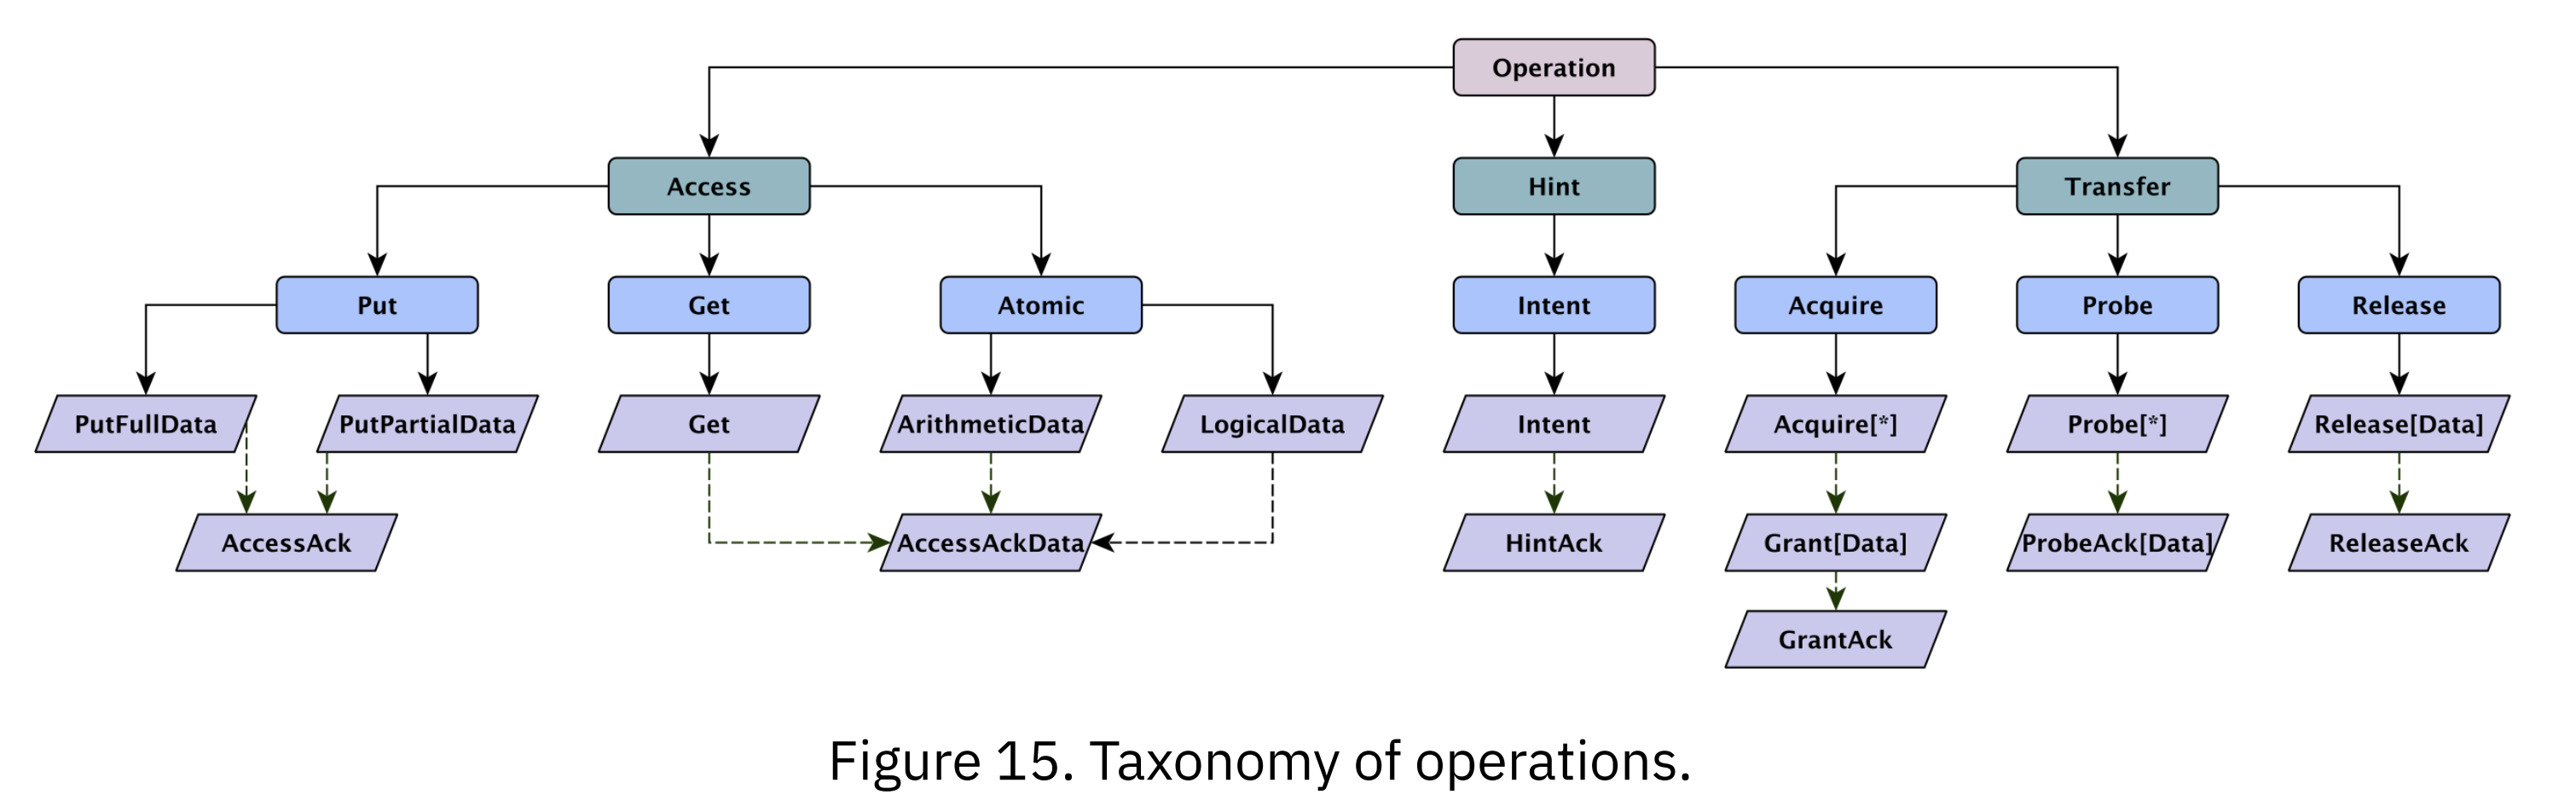
\includegraphics[width=\textwidth]{Img/TileLink_Operations.PNG} %插入图片,[]中设置图片大小,{}中是图片文件名
\caption{Taxonomy of operations} %最终文档中希望显示的图片标题
\label{TileLink_Operations} %用于文内引用的标签
\end{figure}

\paragraph{Get操作}
Get操作是master对slave发起uncache的读,master只需要数据,而不需要缓存这个数据的权限。Get操作请求由master通过A通道发送Get消息,确认信息由slave通过D通道发送AccessAckData消息。

\paragraph{Put操作}
Put操作是master对slave发起uncache的写,master只需要把新数据写进slave就可以了,而不需要缓存这个数据的权限。Put操作请求由master通过A通道发送PutFullData或者PutPartialData消息,确认信息由slave通过D通道发送AccessAck消息。

\paragraph{Acquire操作}
Acquire操作是master对slave发起的申请块权限的操作。当操作完成后,master将获得块的特定权限,它将可以将数据块缓存在本地,并在本地执行权限允许的读写操作。
Acquire操作包含三步:
\begin{enumerate}
	\item master向slave发送Acquire消息,对于特定数据块申请特定的权限。
	\item slave向master回复Grant[Data]消息,对于此数据块,赋予master特定的权限(此权限可能比master请求的权限更高)。
	\item master使用GrantAck响应消息来提供对事务完成的最终确认。
\end{enumerate}

\paragraph{Probe操作}
Probe操作是slave对master发起的块权限查询或修改操作。当操作完成后,master将失去块的部分或全部权限。
Probe操作包含两步:首先slave向master发送ProbeBlock或ProbePerm消息,表明它希望将master缓存的特定数据块的降至特定的权限。接着,master回复ProbeAck[Data]来确认此消息,并写回可能的脏数据。

\paragraph{Release操作}
Release操作是master对slave发起的,主动的释放块权限和数据的操作。当操作完成后,master将失去块的部分或全部权限。
Release操作包含两步:首先master向slave发送Release[Data]消息,表明它将自己缓存的特定数据块降至特定的权限,同时写回可能有的脏数据。接着,slave回复ReleaseAck来确定此消息。

\section{TileLink与一致性协议}

在前面的小节中,我们介绍了TileLink中有哪些通道,哪些消息,哪些操作,其中有些就是和维护一致性有关的。在这一小节,我们完整介绍TileLink协议是如何维护一致性的。包括TileLink定义的块的权限,权限的转移以及操作定序等。
TileLink定义了缓存的数据块的权限包括None,Read以及Read + Write。
在TileLink中,对于一个数据块的所有缓存将构成了一棵树。树的根节点都位于缓存数据块的最终存储位置,例如DDR。根据节点在树中的不同位置,可以划分为四类:
\begin{itemize}
	\item Nothing:当前不缓存数据副本的节点,没有读取或写入权限。
	\item Trunk:在Tip和根节点之间的路径上具有缓存副本的节点。这类节点既没有读权限也没有写权限。例如,当写权限位于L1时,其下面的L2和L3就位于L1到根节点DDR的路径上,L2和L3就处于Trunk状态。
	\item Tip:缓存了数据副本节点,拥有最高权限,是负责对读写请求序列化的点。此状态下拥有对其副本的读/写权限,其中可能包含脏数据。
	\item Branch:在Tip上方的具有缓存副本的节点。对其副本具有只读权限。
\end{itemize}

下面我们可以简单对比一下TileLink协议的状态和MESI的状态,上述四种状态,无法严格对应到MESI协议,但大部分是可以对应过去的。
MESI协议中有四种状态,分别是:
\begin{itemize}
	\item Modified (M)
	\item Exclusive (E)
	\item Shared (S)
	\item Invalid (I)
\end{itemize}

Nothing和Invalid,Branch和Shared是可以一一对应的。Tip对应于Modified和Exclusive状态。TileLink在设计上,并不需要其他节点区分拥有写权限的节点有没有修改过数据,是不是dirty的。它们只需要只需要知道那个节点拥有最高权限就可以。至于是否修改过数据,只有那个节点自己需要关心,拥有最高权限的节点,可以自己内部设计有dirty bit,来记录自己有没有修改过数据,并根据这个bit来判断自己要不要写回脏数据。
Trunk状态是TileLink所独有的,这与TileLink的一致性协议设计是有关的。TileLink要求对于任何一块被缓存的数据块,所有缓存了它的节点必须组成一棵树,称为coherence tree。由于TileLink网络是有向无环图,同时被缓存的数据块唯一来自一个根节点(如DDR),需要组成树,实际上要求下级cache对上一级cache保持Inclusive的关系。这并不是说TileLink要求所有的cache都必须被设计成Inclusive Cache。下一级Cache并不需要真的缓存这个数据块,但是它需要知道自己处于Trunk状态,并且自己的子节点缓存了这个块。

在TileLink的网络中,节点之间通过执行权限转移操作,保证了数据的一致性以及对数据写的定序。
一般来说:
Acquire操作用来主动申请权限。
而Release操作用来主动地降低权限(例如当cache发生了替换,需要写时)。
Probe操作是一致性的invalidate请求,用来降低client的权限。

下面我们以一组例子说明在TileLink网络中,一致性是如何维护的:
\begin{figure}[H] %H为当前位置,!htb为忽略美学标准,htbp为浮动图形
\centering %图片居中
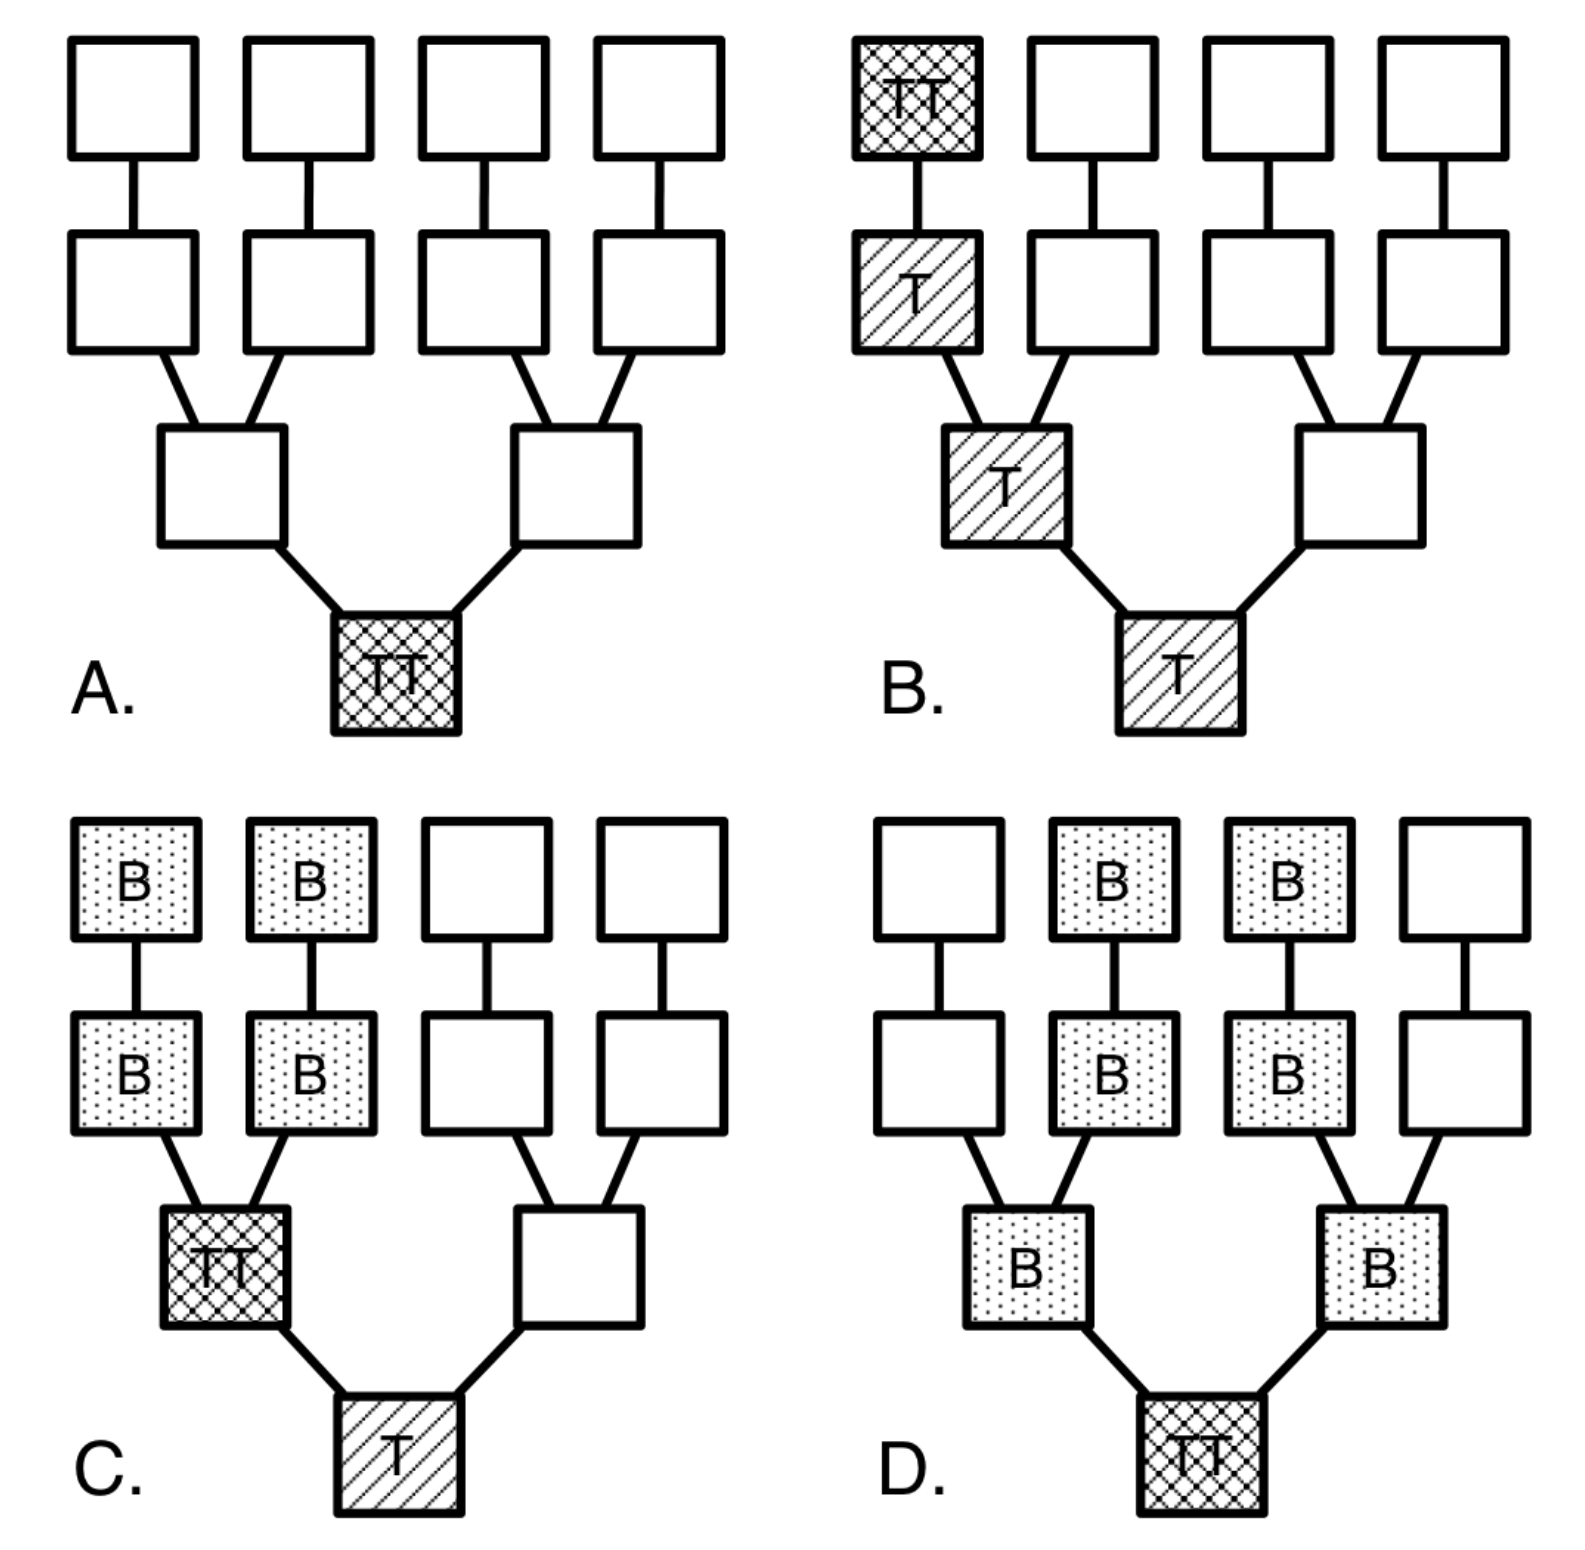
\includegraphics[width=\textwidth]{Img/TileLink_coherence.PNG} %插入图片,[]中设置图片大小,{}中是图片文件名
\caption{TileLink coherence examples} %最终文档中希望显示的图片标题
\label{TileLink_coherence} %用于文内引用的标签
\end{figure}

图中的树描述了一个系统中的多个缓存节点。最下方是DDR,最上方是L1 Cache。缓存了某个特定数据块的所有缓存节点构成了一棵树,以DDR为树根。
假设这是针对某个数据块d1的coherence tree。
图中的状态标识是:空白指Nothing状态,B指Branch状态,T指Trunk状态,TT是Tip状态。
L1 Cache从左到右标号分别为0,1,2,3。
L2 Cache从左到右标号分别为0,1,2,3。
L3 Cache从左到右标号分别为0,1。

图A到D,展示了系统中针对数据块d1的coherence tree的变化过程。

\begin{enumerate}
	\item 开始时,在图A的状态下,数据块d1存在于DDR中,系统中的其他cache都没有缓存d1,因此DDR节点是TT状态。
	\item L1 0请求了d1的写权限,因此从L1 0开始逐级向下通过Acquire操作升级权限,最终Tip状态从DDR转移到了L1 Cache 0,路径上的其他节点都变成了Trunk状态。Coherence Tree演化为了图B状态。
	\item L1 1通过Acquire申请d1的读权限,L2 1也向下转发请求,Acquire请求到达L3 0。L3 0发现自己处于Trunk状态,意味着它的某个孩子节点拥有Tip状态。因此L3 0向L2 0发送ProbeBlock请求,L2 0发现自己也是Trunk状态,因此将ProbeBlock向上发送到L1 0。L1 0收到ProbeBlock请求后,通过ProbeAckData消息将自己的权限降为Branch,并将脏数据写回到L2 0。L2 0也将ProbeAckData发送到L3 0,L2 0变为Branch状态。L3 0收到ProbeAckData后,回收了针对d1数据块的Tip权限,并通过GrantData,将数据和权限发送到L2 1,进而上传到L1 1,它们变为了Branch状态。Coherence Tree演化到了图C状态。
	\item L1 2通过Acquire申请d1的读权限,与前一步一样,最终Tip权限回到了DDR。值得注意的是,在图D中,L1 0和L2 0的Branch状态消失了,这不是L1 2的读导致的,可能是它们自己释放导致的。最终,Coherence Tree演化为了图D。
\end{enumerate}

\section{Verification}

随着系统复杂性的提升,流片成本的增加,如何保证芯片设计实现完整地达到功能与性能要求,没有设计或实现的漏洞,成为了非常关键的问题。验证应运而生。功能验证是在流片前验证开发设计是否遵守给定规格的工作,在芯片全流程中占据关键位置。如今,验证是设计过程中的基本步骤,它比设计实现需要更高的资源,甚至高达30%到40%的项目资源。

本节介绍功能验证的基本流程以及基本方法。

#### Verification的基础知识

首先验证是什么东西,验证是在干什么。

Verification的重要性。

验证的流程:specification(功能详述),验证计划,开发验证环境,测试,回归测试,芯片生产,硅后系统测试,逃逸分析。
本验证工作主要关注的是硅前的阶段,即在流片前协助调试,尽可能地发现bug。

验证的层次

Functional Verification是在做什么东西。
有哪些验证的方法,各有什么优缺点。

动态验证
静态验证

现在大家常用的验证方法。

#### UVM验证方法学

UVM是什么东西。是用来产生testbench的一种方法学。
UVM structure。

\chapter{设计}\label{chap:design}

\section{TileLink一致性协议}

\begin{figure}[H] %H为当前位置,!htb为忽略美学标准,htbp为浮动图形
\centering %图片居中
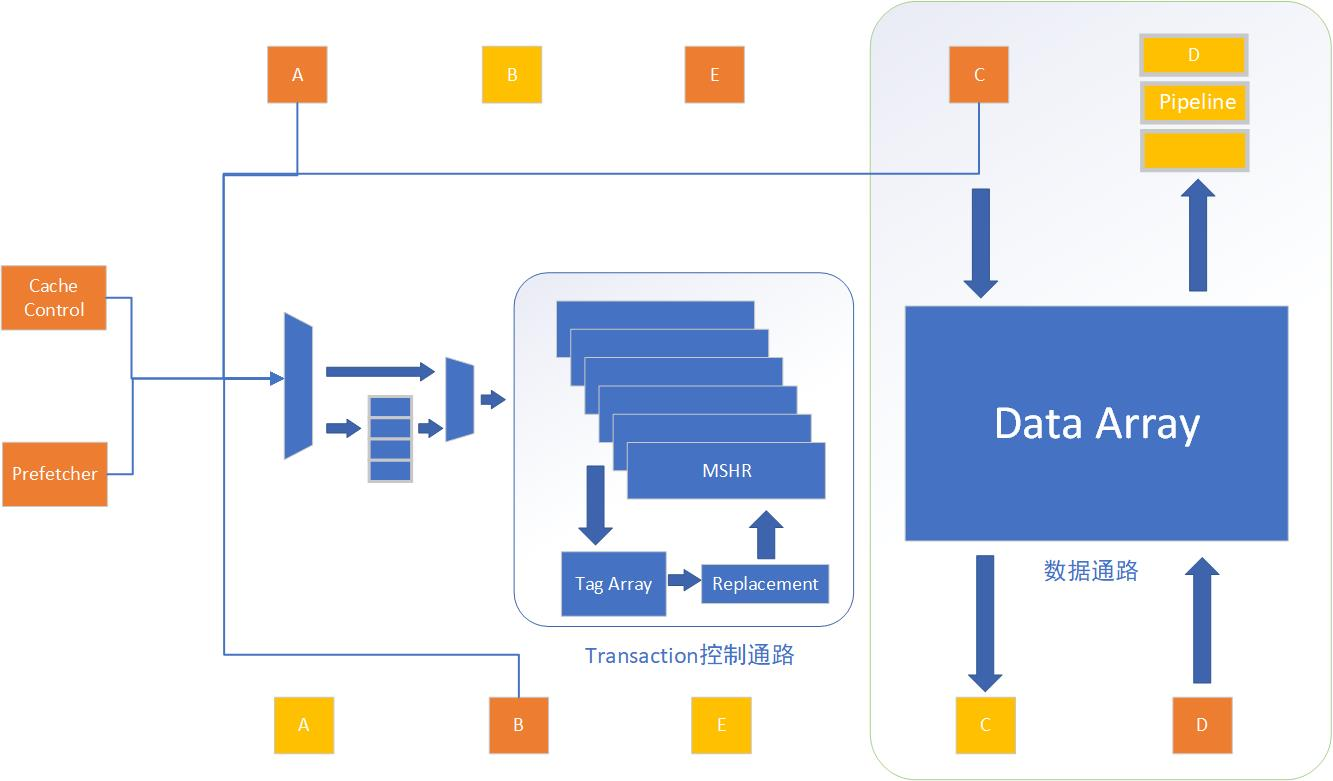
\includegraphics[width=\textwidth]{Img/BlockInclusiveCache.jpg} %插入图片,[]中设置图片大小,{}中是图片文件名
\caption{BlockInclusiveCache} %最终文档中希望显示的图片标题
\label{BlockInclusiveCache} %用于文内引用的标签
\end{figure}

\begin{figure}[H] %H为当前位置,!htb为忽略美学标准,htbp为浮动图形
\centering %图片居中
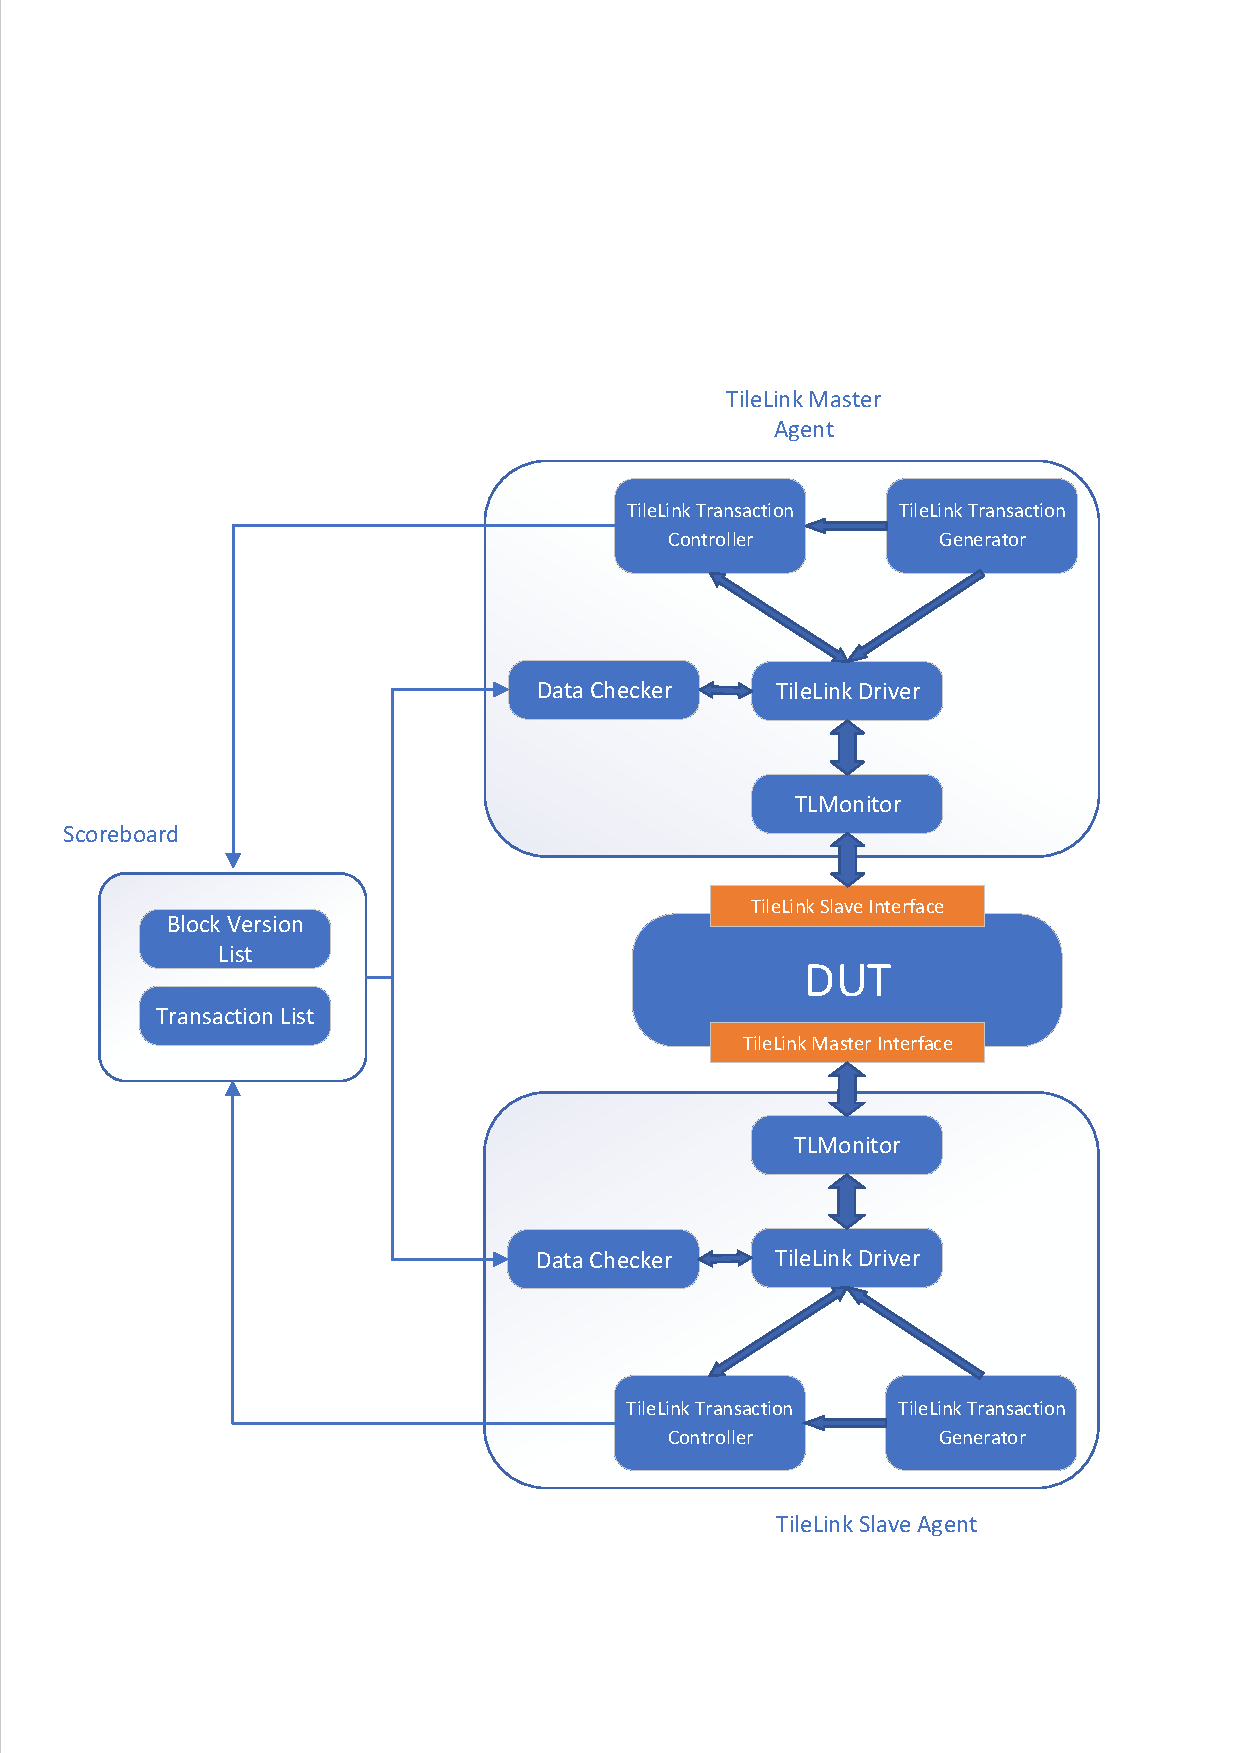
\includegraphics[width=\textwidth]{Img/BlockInclusiveCacheTest.pdf} %插入图片,[]中设置图片大小,{}中是图片文件名
\caption{BlockInclusiveCacheTest} %最终文档中希望显示的图片标题
\label{BlockInclusiveCacheTest} %用于文内引用的标签
\end{figure}

%---------------------------------------------------------------------------%
% main content
%-
%-> Appendix
%-
\cleardoublepage%
\appendix% initialize the environment
\chapter{中国科学院大学学位论文撰写要求}

学位论文是研究生科研工作成果的集中体现,是评判学位申请者学术水平、授予其学位的主要依据,是科研领域重要的文献资料。根据《科学技术报告、学位论文和学术论文的编写格式》(GB/T 7713-1987)、《学位论文编写规则》(GB/T 7713.1-2006)和《文后参考文献著录规则》(GB7714—87)等国家有关标准,结合中国科学院大学(以下简称“国科大”)的实际情况,特制订本规定。

\section{论文无附录者无需附录部分}

\section{测试公式编号 \texorpdfstring{$\Lambda,\lambda,\theta,\bar{\Lambda},\sqrt{S_{NN}}$}{$\textLambda,\textlambda,\texttheta,\bar{\textLambda},\sqrt{S_{NN}}$}} \label{sec:testmath}

\begin{equation} \label{eq:appedns}
    \adddotsbeforeeqnnum%
    \begin{cases}
        \frac{\partial \rho}{\partial t} + \nabla\cdot(\rho\Vector{V}) = 0\\
        \frac{\partial (\rho\Vector{V})}{\partial t} + \nabla\cdot(\rho\Vector{V}\Vector{V}) = \nabla\cdot\Tensor{\sigma}\\
        \frac{\partial (\rho E)}{\partial t} + \nabla\cdot(\rho E\Vector{V}) = \nabla\cdot(k\nabla T) + \nabla\cdot(\Tensor{\sigma}\cdot\Vector{V})
    \end{cases}
\end{equation}
\begin{equation}
    \adddotsbeforeeqnnum%
    \frac{\partial }{\partial t}\int\limits_{\Omega} u \, \mathrm{d}\Omega + \int\limits_{S} \unitVector{n}\cdot(u\Vector{V}) \, \mathrm{d}S = \dot{\phi}
\end{equation}
\[
    \begin{split}
        \mathcal{L} \{f\}(s) &= \int _{0^{-}}^{\infty} f(t) e^{-st} \, \mathrm{d}t, \ 
        \mathscr{L} \{f\}(s) = \int _{0^{-}}^{\infty} f(t) e^{-st} \, \mathrm{d}t\\
        \mathcal{F} {\bigl (} f(x+x_{0}) {\bigr )} &= \mathcal{F} {\bigl (} f(x) {\bigr )} e^{2\pi i\xi x_{0}}, \ 
        \mathscr{F} {\bigl (} f(x+x_{0}) {\bigr )} = \mathscr{F} {\bigl (} f(x) {\bigr )} e^{2\pi i\xi x_{0}}
    \end{split}
\]

mathtext: $A,F,L,2,3,5,\sigma$, mathnormal: $A,F,L,2,3,5,\sigma$, mathrm: $\mathrm{A,F,L,2,3,5,\sigma}$.

mathbf: $\mathbf{A,F,L,2,3,5,\sigma}$, mathit: $\mathit{A,F,L,2,3,5,\sigma}$, mathsf: $\mathsf{A,F,L,2,3,5,\sigma}$.

mathtt: $\mathtt{A,F,L,2,3,5,\sigma}$, mathfrak: $\mathfrak{A,F,L,2,3,5,\sigma}$, mathbb: $\mathbb{A,F,L,2,3,5,\sigma}$.

mathcal: $\mathcal{A,F,L,2,3,5,\sigma}$, mathscr: $\mathscr{A,F,L,2,3,5,\sigma}$, boldsymbol: $\boldsymbol{A,F,L,2,3,5,\sigma}$.

vector: $\Vector{\sigma, T, a, F, n}$, unitvector: $\unitVector{\sigma, T, a, F, n}$

matrix: $\Matrix{\sigma, T, a, F, n}$, unitmatrix: $\unitMatrix{\sigma, T, a, F, n}$

tensor: $\Tensor{\sigma, T, a, F, n}$, unittensor: $\unitTensor{\sigma, T, a, F, n}$ 

\section{测试生僻字}

霜蟾盥薇曜灵霜颸妙鬘虚霩淩澌菀枯菡萏泬寥窅冥毰毸濩落霅霅便嬛岧峣瀺灂姽婳愔嫕飒纚棽俪緸冤莩甲摛藻卮言倥侗椒觞期颐夜阑彬蔚倥偬澄廓簪缨陟遐迤逦缥缃鹣鲽憯懔闺闼璀错媕婀噌吰澒洞阛闠覼缕玓瓑逡巡諓諓琭琭瀌瀌踽踽叆叇氤氲瓠犀流眄蹀躞赟嬛茕頔璎珞螓首蘅皋惏悷缱绻昶皴皱颟顸愀然菡萏卑陬纯懿犇麤掱暒 墌墍墎墏墐墒墒墓墔墕墖墘墖墚墛坠墝增墠墡墢墣墤墥墦墧墨墩墪樽墬墭堕墯墰墱墲坟墴墵垯墷墸墹墺墙墼墽垦墿壀壁壂壃壄壅壆坛壈壉壊垱壌壍埙壏壐壑壒压壔壕壖壗垒圹垆壛壜壝垄壠壡坜壣壤壥壦壧壨坝塆圭嫶嫷嫸嫹嫺娴嫼嫽嫾婳妫嬁嬂嬃嬄嬅嬆嬇娆嬉嬊娇嬍嬎嬏嬐嬑嬒嬓嬔嬕嬖嬗嬘嫱嬚嬛嬜嬞嬟嬠嫒嬢嬣嬥嬦嬧嬨嬩嫔嬫嬬奶嬬嬮嬯婴嬱嬲嬳嬴嬵嬶嬷婶嬹嬺嬻嬼嬽嬾嬿孀孁孂娘孄孅孆孇孆孈孉孊娈孋孊孍孎孏嫫婿媚嵭嵮嵯嵰嵱嵲嵳嵴嵵嵶嵷嵸嵹嵺嵻嵼嵽嵾嵿嶀嵝嶂嶃崭嶅嶆岖嶈嶉嶊嶋嶌嶍嶎嶏嶐嶑嶒嶓嵚嶕嶖嶘嶙嶚嶛嶜嶝嶞嶟峤嶡峣嶣嶤嶥嶦峄峃嶩嶪嶫嶬嶭崄嶯嶰嶱嶲嶳岙嶵嶶嶷嵘嶹岭嶻屿岳帋巀巁巂巃巄巅巆巇巈巉巊岿巌巍巎巏巐巑峦巓巅巕岩巗巘巙巚帠帡帢帣帤帨帩帪帬帯帰帱帲帴帵帷帹帺帻帼帽帾帿幁幂帏幄幅幆幇幈幉幊幋幌幍幎幏幐幑幒幓幖幙幚幛幜幝幞帜幠幡幢幤幥幦幧幨幩幪幭幮幯幰幱庍庎庑庖庘庛庝庠庡庢庣庤庥庨庩庪庬庮庯庰庱庲庳庴庵庹庺庻庼庽庿廀厕廃厩廅廆廇廋廌廍庼廏廐廑廒廔廕廖廗廘廙廛廜廞庑廤廥廦廧廨廭廮廯廰痈廲廵廸廹廻廼廽廿弁弅弆弇弉弖弙弚弜弝弞弡弢弣弤弨弩弪弫弬弭弮弰弲弪弴弶弸弻弼弽弿彖彗彘彚彛彜彝彞彟彴彵彶彷彸役彺彻彽彾佛徂徃徆徇徉后徍徎徏径徒従徔徕徖徙徚徛徜徝从徟徕御徢徣徤徥徦徧徨复循徫旁徭微徯徰徱徲徳徴徵徶德徸彻徺忁忂惔愔忇忈忉忔忕忖忚忛応忝忞忟忪挣挦挧挨挩挪挫挬挭挮挰掇授掉掊掋掍掎掐掑排掓掔掕挜掚挂掜掝掞掟掠采探掣掤掦措掫掬掭掮掯掰掱掲掳掴掵掶掸掹掺掻掼掽掾掿拣揁揂揃揅揄揆揇揈揉揊揋揌揍揎揑揓揔揕揖揗揘揙揤揥揦揧揨揫捂揰揱揲揳援揵揶揷揸揻揼揾揿搀搁搂搃搄搅搇搈搉搊搋搌搎搏搐搑搒摓摔摕摖摗摙摚摛掼摝摞摠摡斫斩斮斱斲斳斴斵斶斸旪旫旮旯晒晓晔晕晖晗晘晙晛晜晞晟晠晡晰晣晤晥晦晧晪晫晬晭晰晱晲晳晴晵晷晸晹晻晼晽晾晿暀暁暂暃暄暅暆暇晕晖暊暋暌暍暎暏暐暑暒暓暔暕暖暗旸暙暚暛暜暝暞暟暠暡暣暤暥暦暧暨暩暪暬暭暮暯暰昵暲暳暴暵
% appendix content
%-
%-> Backmatter: bibliography, glossary, index
%-
\backmatter% initialize the environment
\intotoc*{\cleardoublepage}{\bibname}% add link to toc
\artxifstreq{\artxbib}{bibtex}{% enable bibtex
    \bibliography{Biblio/ref}% bibliography
}{%
    \printbibliography% bibliography
}
%---------------------------------------------------------------------------%
%->> Backmatter
%---------------------------------------------------------------------------%
\chapter{作者简历及攻读学位期间发表的学术论文与研究成果}

\textbf{本科生无需此部分}。

\section*{作者简历}

\subsection*{casthesis作者}

吴凌云,福建省屏南县人,中国科学院数学与系统科学研究院博士研究生。

\subsection*{ucasthesis作者}

莫晃锐,湖南省湘潭县人,中国科学院力学研究所硕士研究生。

\section*{已发表(或正式接受)的学术论文:}

{
\setlist[enumerate]{}% restore default behavior
\begin{enumerate}[nosep]
    \item ucasthesis: A LaTeX Thesis Template for the University of Chinese Academy of Sciences, 2014.
\end{enumerate}
}

\section*{申请或已获得的专利:}

(无专利时此项不必列出)

\section*{参加的研究项目及获奖情况:}

可以随意添加新的条目或是结构。

\chapter[致谢]{致\quad 谢}\chaptermark{致\quad 谢}% syntax: \chapter[目录]{标题}\chaptermark{页眉}
\thispagestyle{noheaderstyle}% 如果需要移除当前页的页眉
%\pagestyle{noheaderstyle}% 如果需要移除整章的页眉

感激casthesis作者吴凌云学长,gbt7714-bibtex-style
开发者zepinglee,和ctex众多开发者们。若没有他们的辛勤付出和非凡工作,\LaTeX{}菜鸟的我是无法完成此国科大学位论文\LaTeX{}模板ucasthesis的。在\LaTeX{}中的一点一滴的成长源于开源社区的众多优秀资料和教程,在此对所有\LaTeX{}社区的贡献者表示感谢!

ucasthesis国科大学位论文\LaTeX{}模板的最终成型离不开以霍明虹老师和丁云云老师为代表的国科大学位办公室老师们制定的官方指导文件和众多ucasthesis用户的热心测试和耐心反馈,在此对他们的认真付出表示感谢。特别对国科大的赵永明同学的众多有效反馈意见和建议表示感谢,对国科大本科部的陆晴老师和本科部学位办的丁云云老师的细致审核和建议表示感谢。谢谢大家的共同努力和支持,让ucasthesis为国科大学子使用\LaTeX{}撰写学位论文提供便利和高效这一目标成为可能。

\cleardoublepage[plain]% 让文档总是结束于偶数页,可根据需要设定页眉页脚样式,如 [noheaderstyle]
%---------------------------------------------------------------------------%
% other information
\end{document}
%---------------------------------------------------------------------------%

